\vspace{-6mm}
\section{}
실험 1에서는 SimuLTE를 통해 하나의 LTE 기지국(eNodeB)과 이를 매개로 통신을 주고 받는 두 개의 단말(UE)로 이루어진 Radio Access Network(RAN)을 구현한다. 실험 1-1에서는 단말 사이의 거리가 증가함에 따라 throughput(received packet 수)가 어떻게 변화하는지, 실험 1-2에서는 네트워크 CQI이 증가함에 따라 throughput(received packet 수)가 어떻게 변화하는지 확인한다.
\subsection*{Experiment 1-1}
    \subsubsection*{1. 1. 1 Code}
    \vspace{-3mm}
            \vspace{-2mm}
            \begin{listing}[h!]
            \inputminted[framerule = 1pt,framesep = 2mm , frame = lines, fontsize=\footnotesize]{c}{./code/week11/Experiment_01/omnet1.cpp}
            \vspace{-3mm}
            \caption{\footnotesize experiment 1-1, omnetpp.ini}
            \end{listing}
            \vspace{-6mm}
    \subsubsection*{1. 1. 2 Simulation}
    \vspace{-3mm}
        omnetpp.ini 파일을 실행시켜 다음과 같은 network를 build 했다. 하나의 eNodeB를 기준으로 좌측에는 TX가, 우측에는 RX가 있다. eNodeB와 단말 사이의 거리를 25m부터 50m까지 5m씩 증가시키면서 실험을 반복했다.
        \begin{figure}[!h]\centering 
	        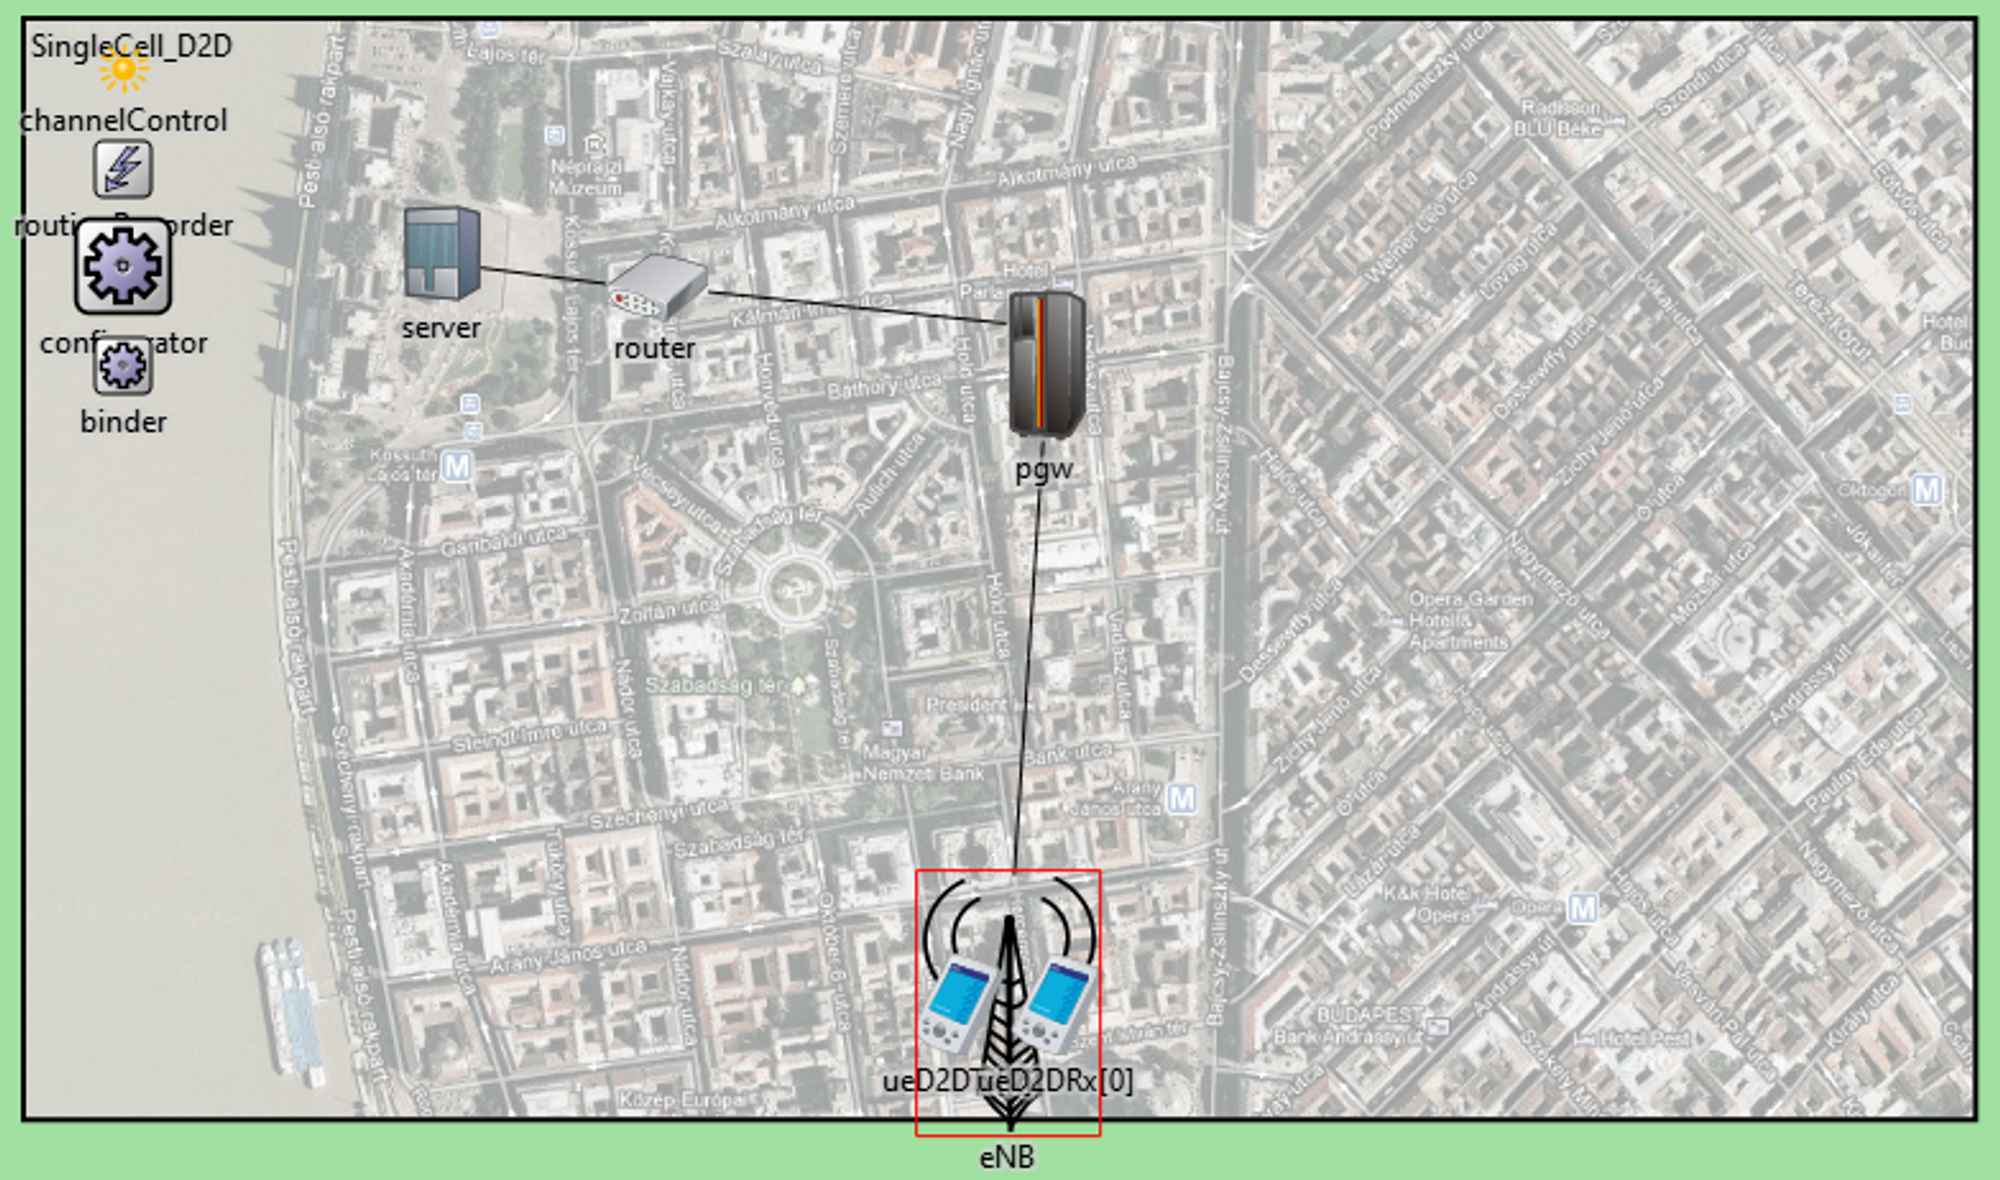
\includegraphics[width=.68\textwidth]{image/week11/1-1-0.png}
	        \caption{\footnotesize
	        experiment 1-1, network simulation}
	        \vspace{-10pt}
        \end{figure}
        
        시뮬레이션 종료 후 생성된 스칼라 데이터 중에서 수신자(ueD2DRx)가 수신한 packetReceived 값을 확인했다. 
            \begin{figure}[h!]
            \centering
            \subfloat[distance: 25m]{
                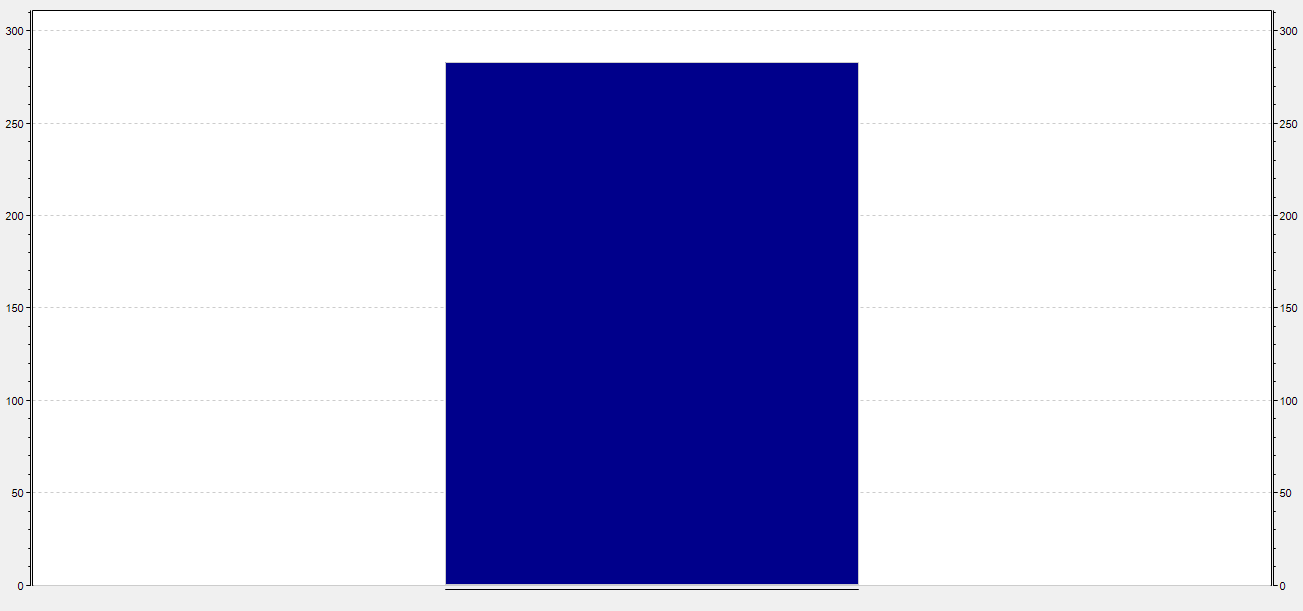
\includegraphics[width=0.30\textwidth]{image/week11/1-1-1.png}
            }\hspace{3mm}
            \subfloat[distance: 30m]{
                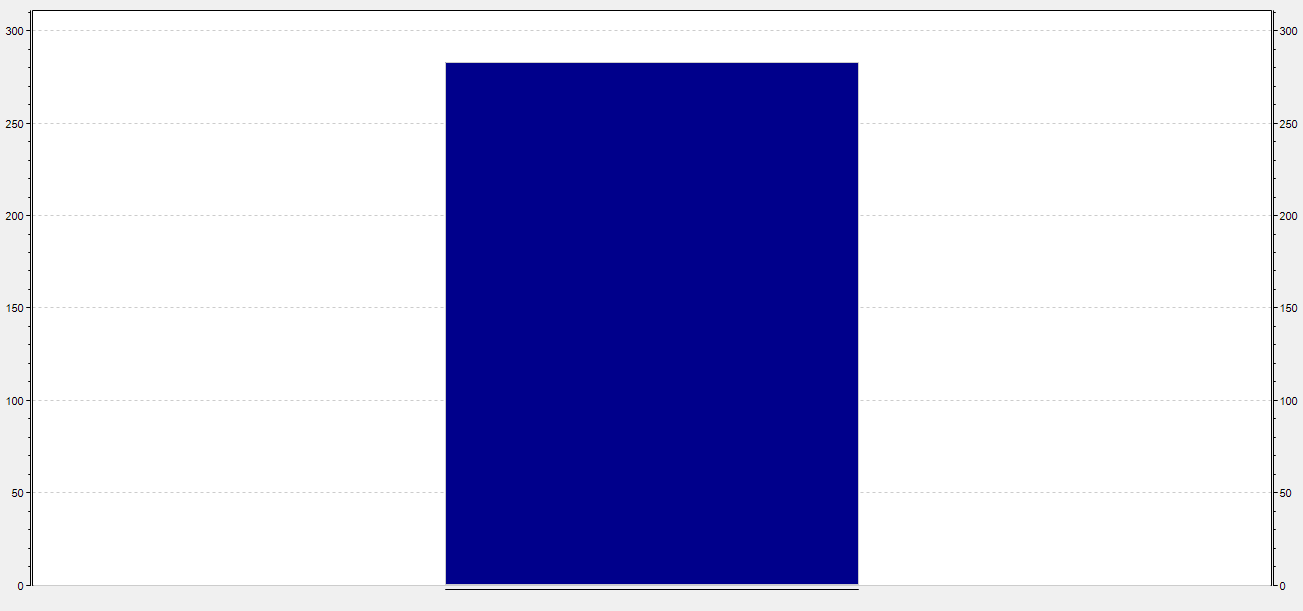
\includegraphics[width=0.30\textwidth]{image/week11/1-1-1.png}
            }\hspace{3mm}
            \subfloat[distance: 35m]{
                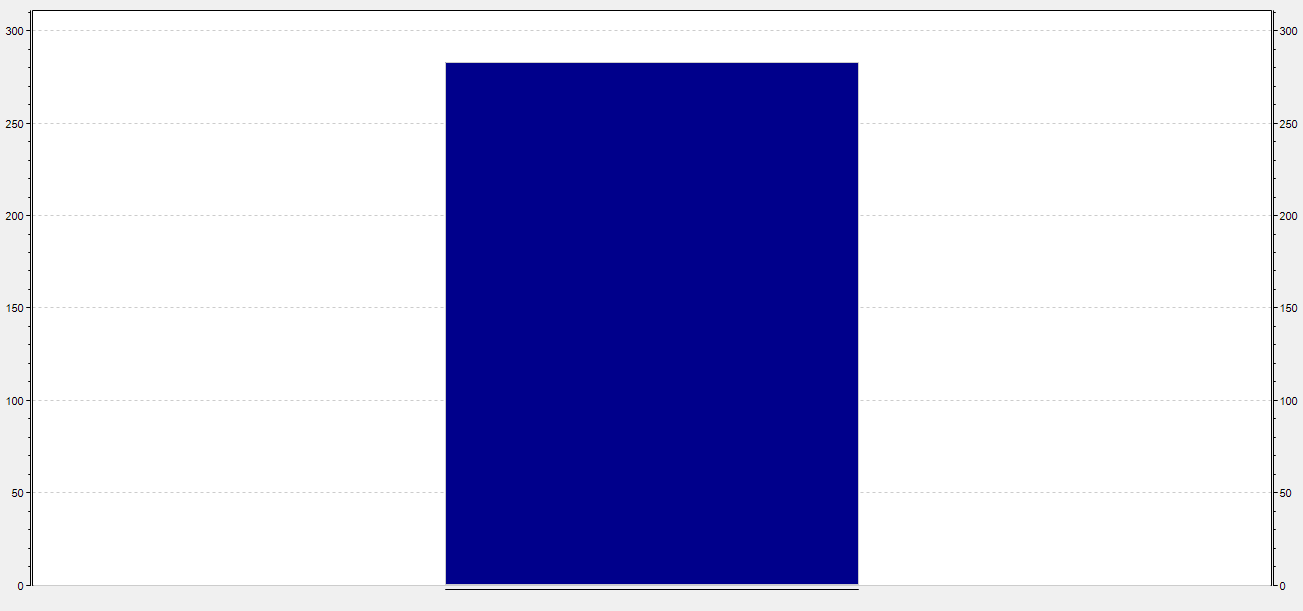
\includegraphics[width=0.30\textwidth]{image/week11/1-1-1.png}
            }\hspace{3mm}
            \subfloat[distance: 40m]{
                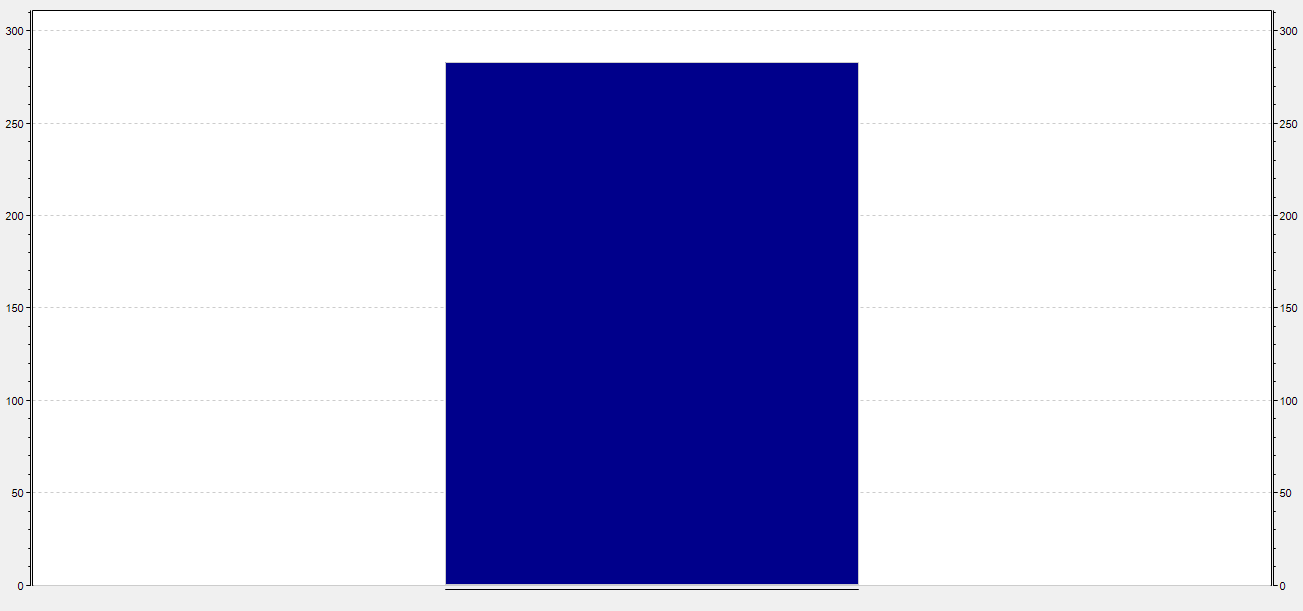
\includegraphics[width=0.30\textwidth]{image/week11/1-1-1.png}
            }\hspace{3mm}
            \subfloat[distance: 45m]{
                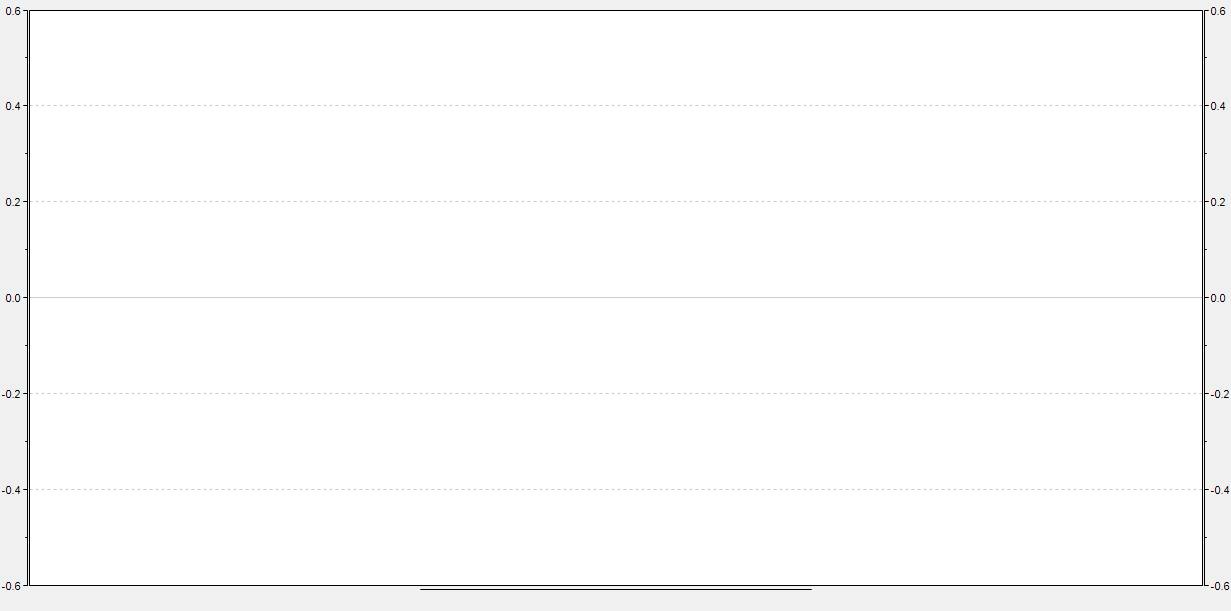
\includegraphics[width=0.30\textwidth]{image/week11/1-1-2.png}
            }\hspace{3mm}
            \subfloat[distance: 50m]{
                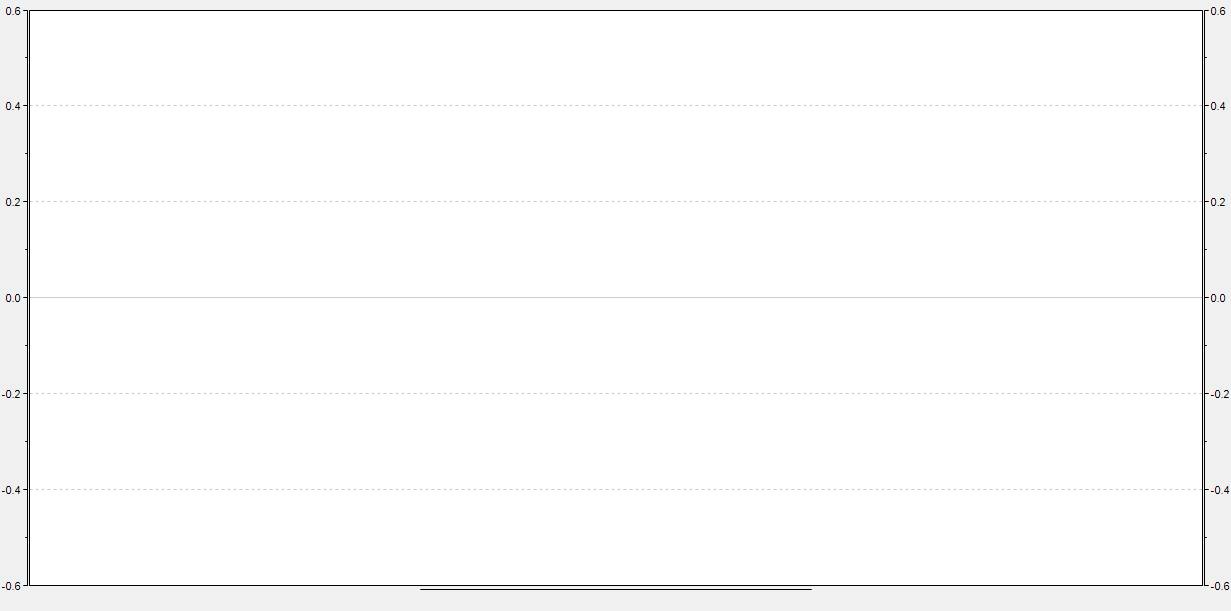
\includegraphics[width=0.30\textwidth]{image/week11/1-1-2.png}
            }\hspace{3mm}
            \caption{Experiment 1-1 Simulation Results Screenshot: packetReceived}
            \end{figure}
    \subsubsection*{1. 1. 3 Discussion}
    \vspace{-3mm}
        시뮬레이션 결과를 다음과 같이 표로 나타냈다.\\
        
        \vspace{-3mm}
        \begin{table}[h!]
        \centering
            \begin{tabular}{|l|l|l|l|l|l|l|}
            \hline
            \textbf{Distance} & 25m & 30m & 35m & 40m & 45m & 50m \\
            \hline
            \multicolumn{1}{|c|}{\textbf{Received Packet}} & \multicolumn{1}{|c|}{283} & 283 & 283 & 283 & 2830 & \multicolumn{1}{|c|}{0} \\
            \hline
            \end{tabular}
            \caption{The nuumber of the packet received with different distances}
        \end{table}
        \vspace{-3mm}
        
        RX가 수신한 packet의 수는 거리가 25m부터 40m까지 283개로 일정하게 유지되다가 45m부터 0으로 감소했다. 모두 같은 CQI 값(1)을 사용했고, 25m부터 40m까지는 모든 packet을 수신할 수 있어 모두 같은 283개의 packet을 수신했다. 거리가 증가함에 따라 SINR이 감소하여 네트워크 상태가 나빠지는데, 45m부터는 정상적인 packet을 수신할 수 없을 정도로 네트워크 상태가 나빠져서 수신한 packet의 수가 0이 된것으로 예상된다. 
        
        %%%%%%%%%%%%%%%%%%%%%%%%%%%%%%%%%%%%%%%%%%%%%%%%%%%
        
\subsection*{Experiment 1-2}
    \subsubsection*{1. 2. 1 Code}
    \vspace{-3mm}
            \vspace{-2mm}
            \begin{listing}[h!]
            \inputminted[framerule = 1pt,framesep = 2mm , frame = lines, fontsize=\footnotesize]{c}{./code/week11/Experiment_01/omnet2.cpp}
            \vspace{-3mm}
            \caption{\footnotesize experiment 1-2, omnetpp.ini}
            \end{listing}
            \vspace{-6mm}
    \subsubsection*{1. 2. 2 Simulation}
    \vspace{-3mm}
        실험 1-1과 같은 네트워크에서 eNodeB와 단말 사이의 거리를 고정시키고 CQI 값을 1, 3, 5, 7, 9로 증가시켰다. CQI 값이 증가함에 따른 received packet 수의 증감에 대한 경향성이  eNodeB와 단말 사이의 거리에 영향을 받는지 확인하기 위해 eNodeB와 단말 사이의 거리를 25m와 30m로 실험을 두번 진행했다. \\
        시뮬레이션 종료 후 생성된 스칼라 데이터 중에서 수신자(ueD2DRx)가 수신한 packetReceived 값을 확인했다.
\newpage
            \begin{figure}[h!]
            \centering
            \subfloat[CQI: 1]{
                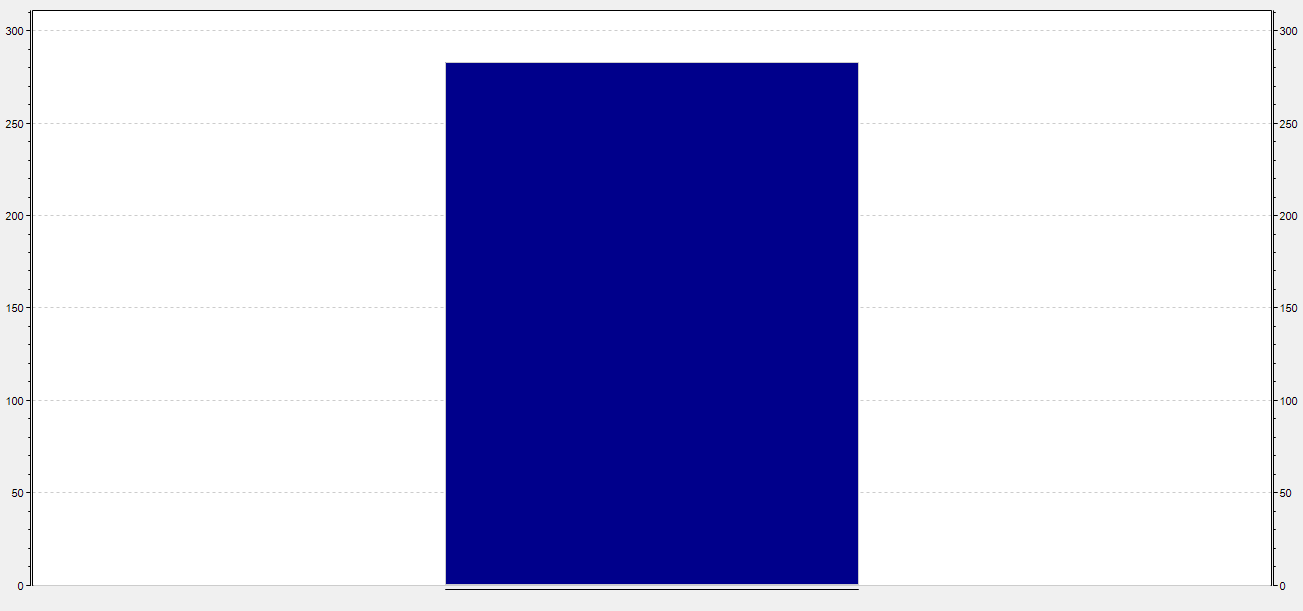
\includegraphics[width=0.30\textwidth]{image/week11/1-2-1.png}
            }\hspace{3mm}
            \subfloat[CQI: 3]{
                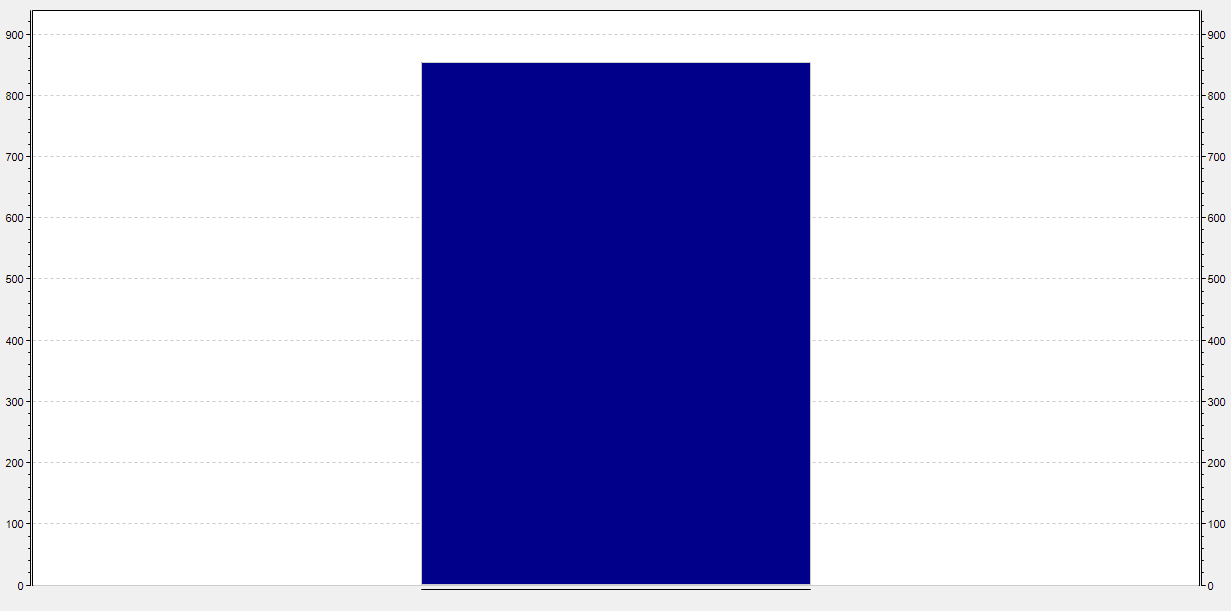
\includegraphics[width=0.30\textwidth]{image/week11/1-2-2.png}
            }\hspace{3mm}
            \subfloat[CQI: 5]{
                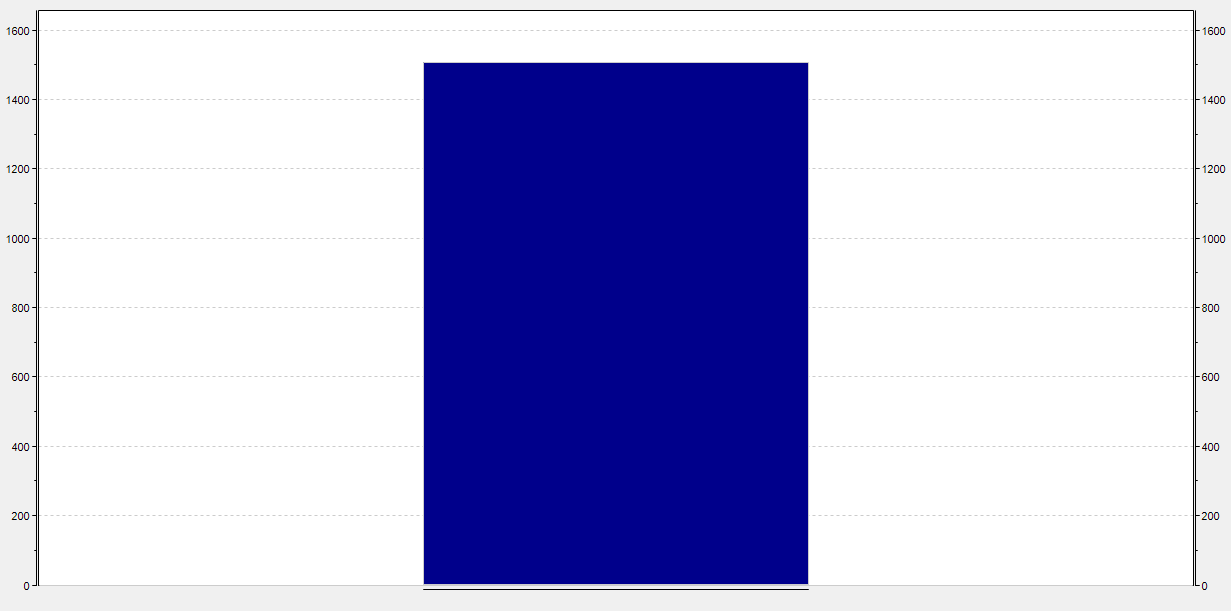
\includegraphics[width=0.30\textwidth]{image/week11/1-2-3.png}
            }\hspace{3mm}
            \subfloat[CQI: 7]{
                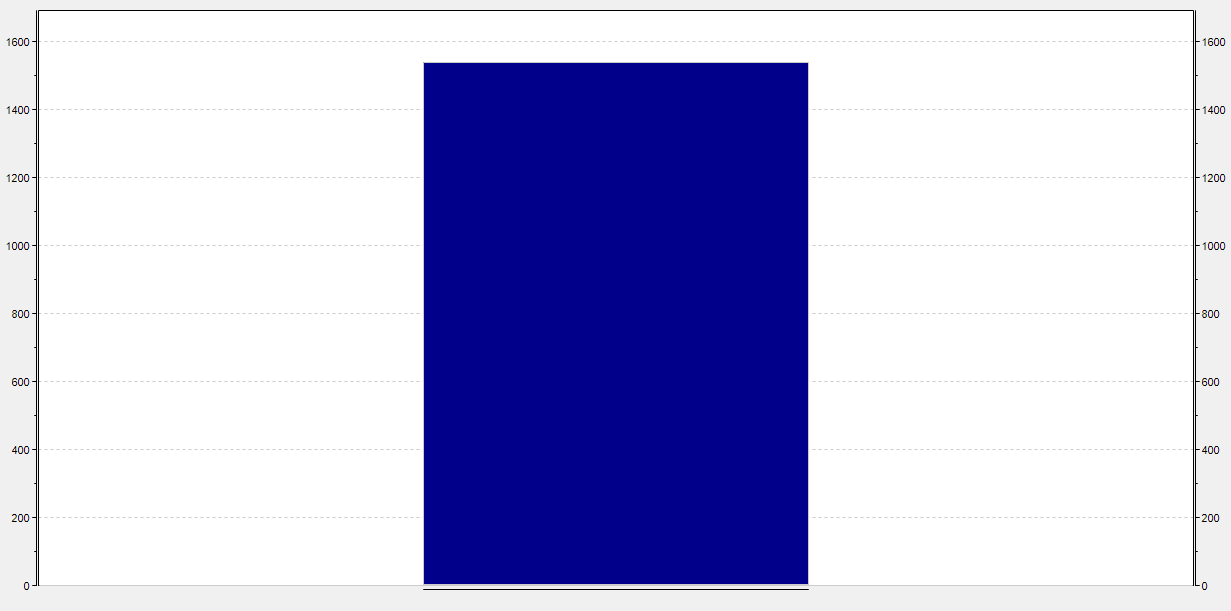
\includegraphics[width=0.30\textwidth]{image/week11/1-2-4.png}
            }\hspace{3mm}
            \subfloat[CQI: 9]{
                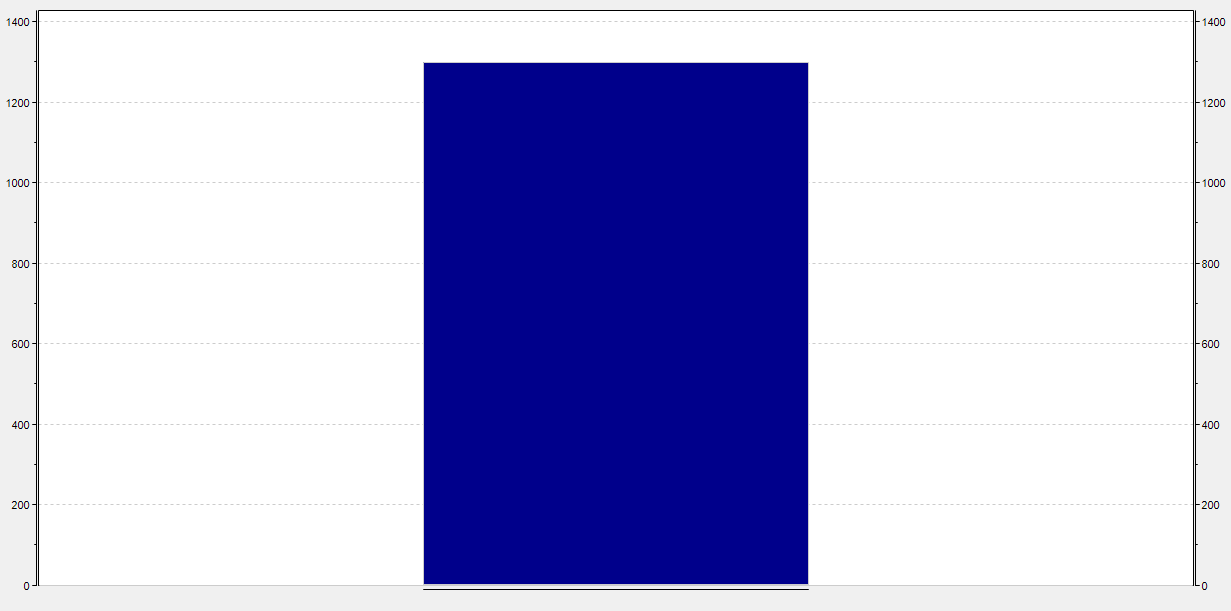
\includegraphics[width=0.30\textwidth]{image/week11/1-2-5.png}
            }\hspace{3mm}
            \caption{Experiment 1-2 Simulation Results Screenshot: 25m, packetReceived}
            \end{figure}
            
            \begin{figure}[h!]
            \centering
            \subfloat[CQI: 1]{
                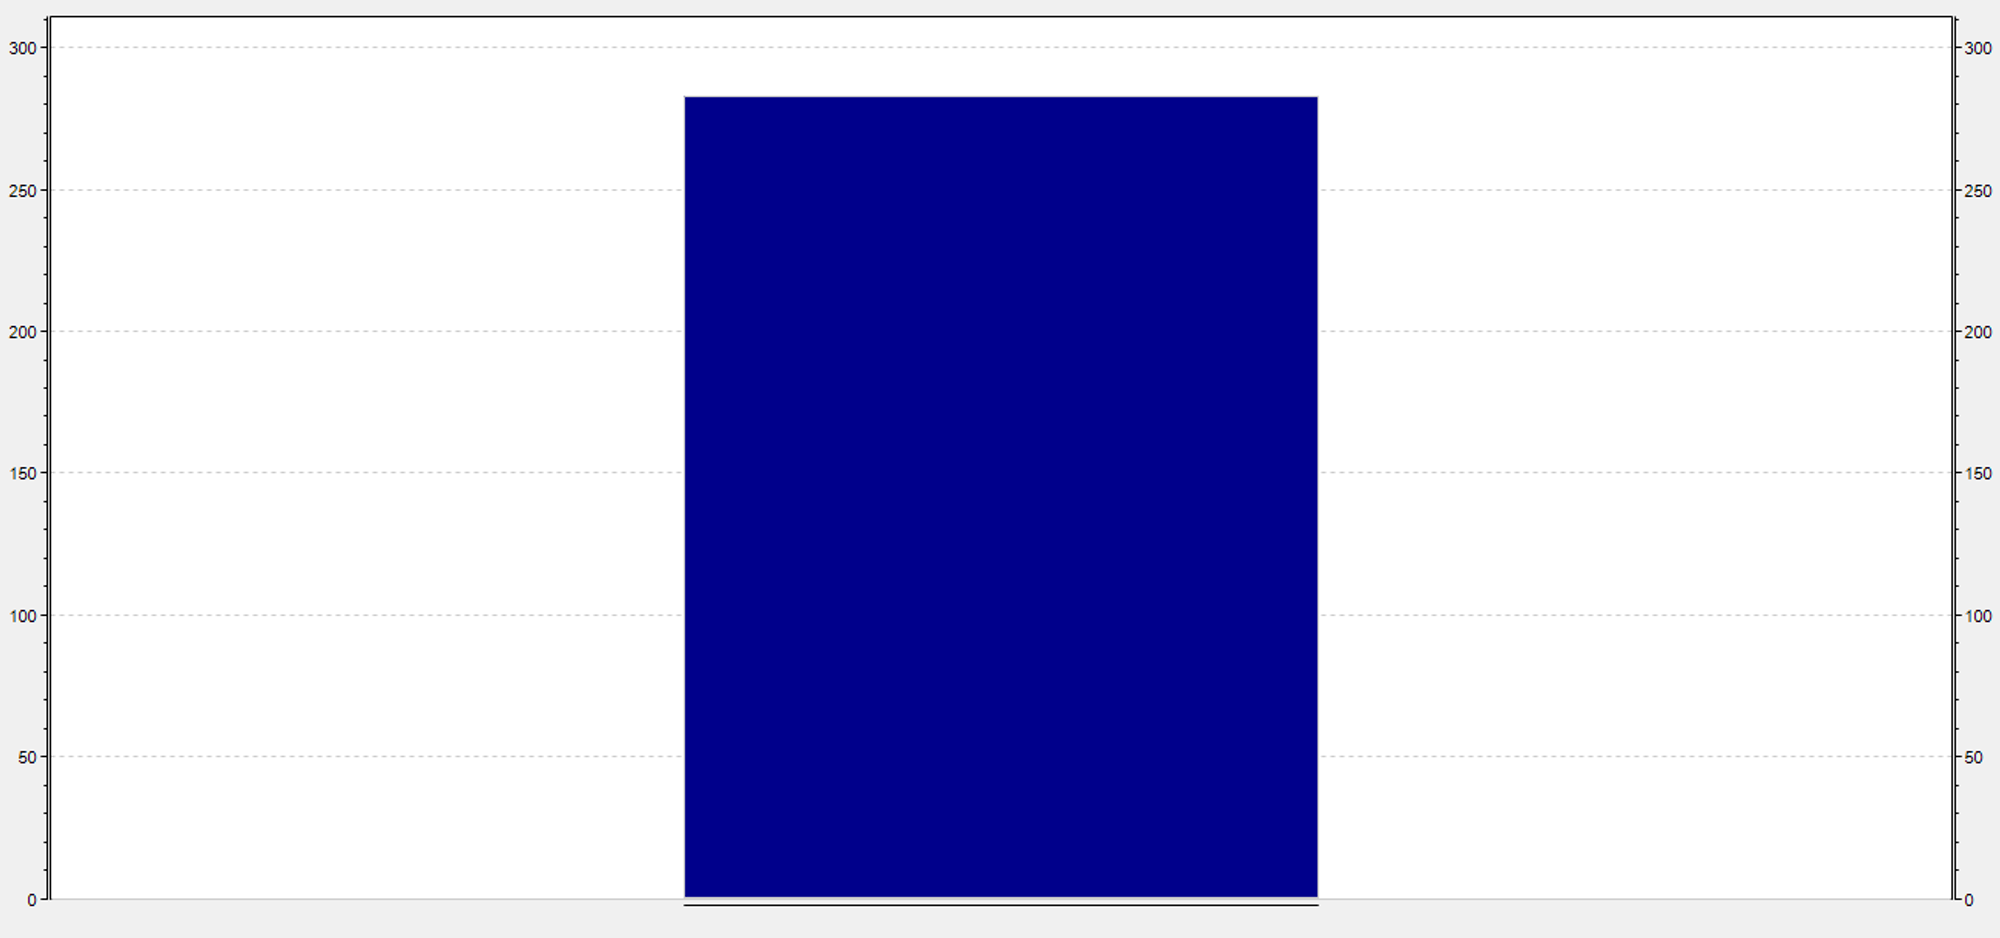
\includegraphics[width=0.30\textwidth]{image/week11/1-2-6.png}
            }\hspace{3mm}
            \subfloat[CQI: 3]{
                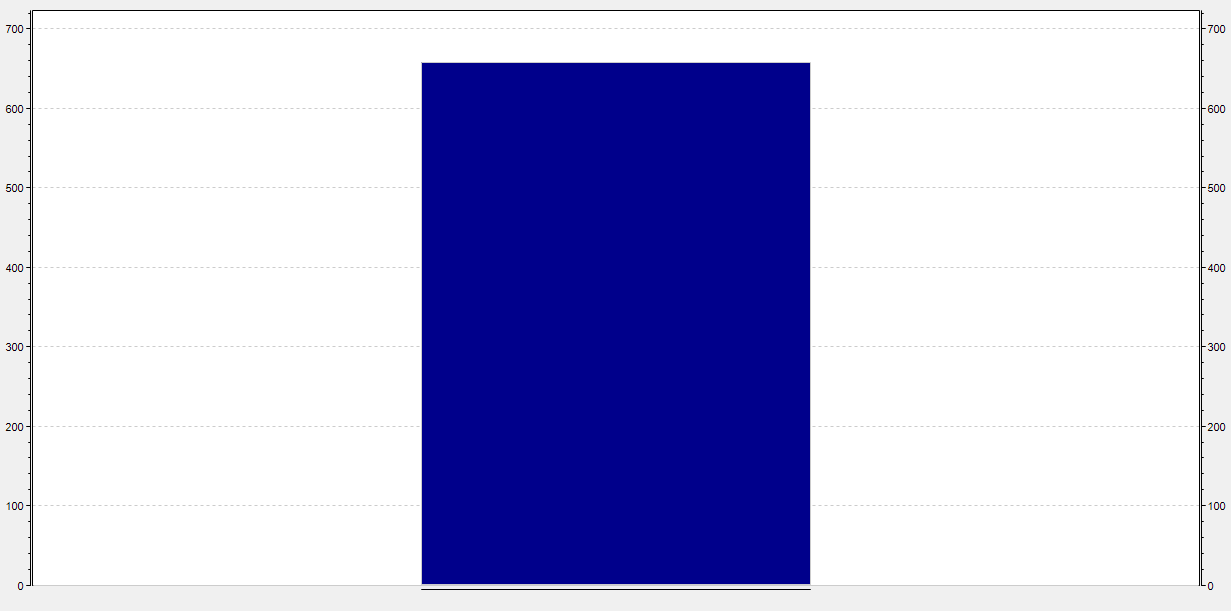
\includegraphics[width=0.30\textwidth]{image/week11/1-2-7.png}
            }\hspace{3mm}
            \subfloat[CQI: 5]{
                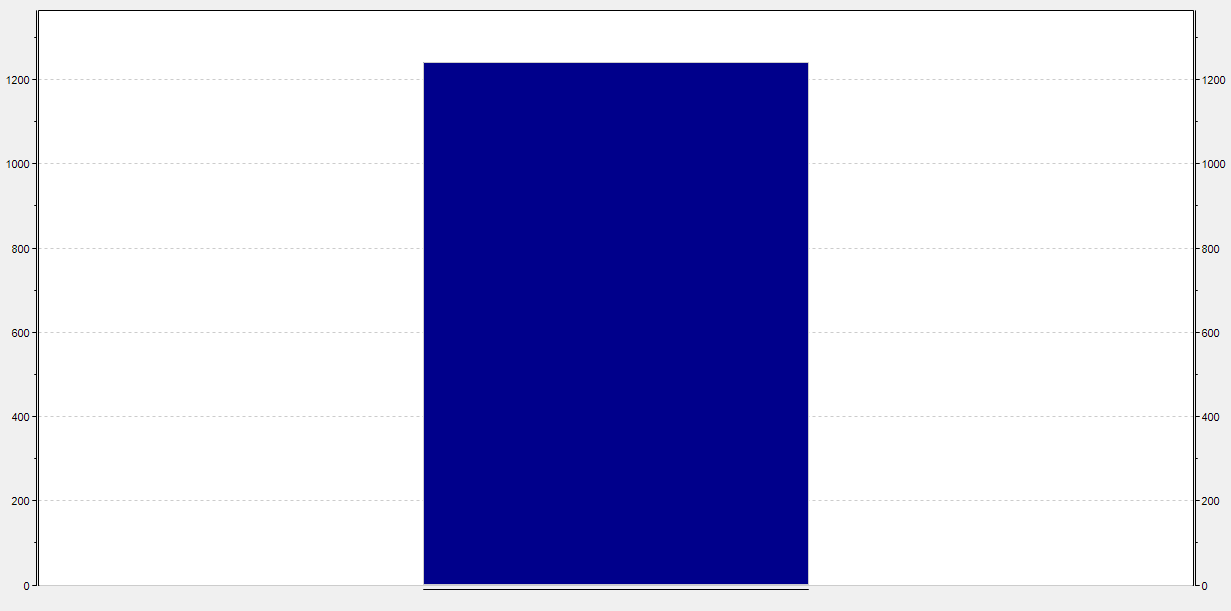
\includegraphics[width=0.30\textwidth]{image/week11/1-2-8.png}
            }\hspace{3mm}
            \subfloat[CQI: 7]{
                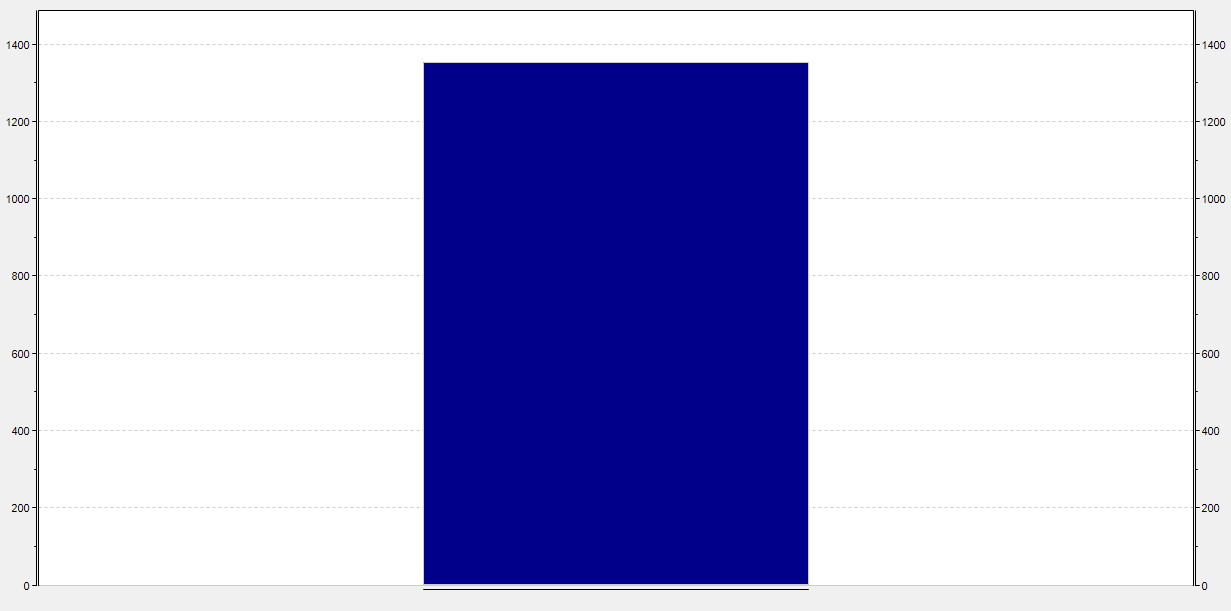
\includegraphics[width=0.30\textwidth]{image/week11/1-2-9.png}
            }\hspace{3mm}
            \subfloat[CQI: 9]{
                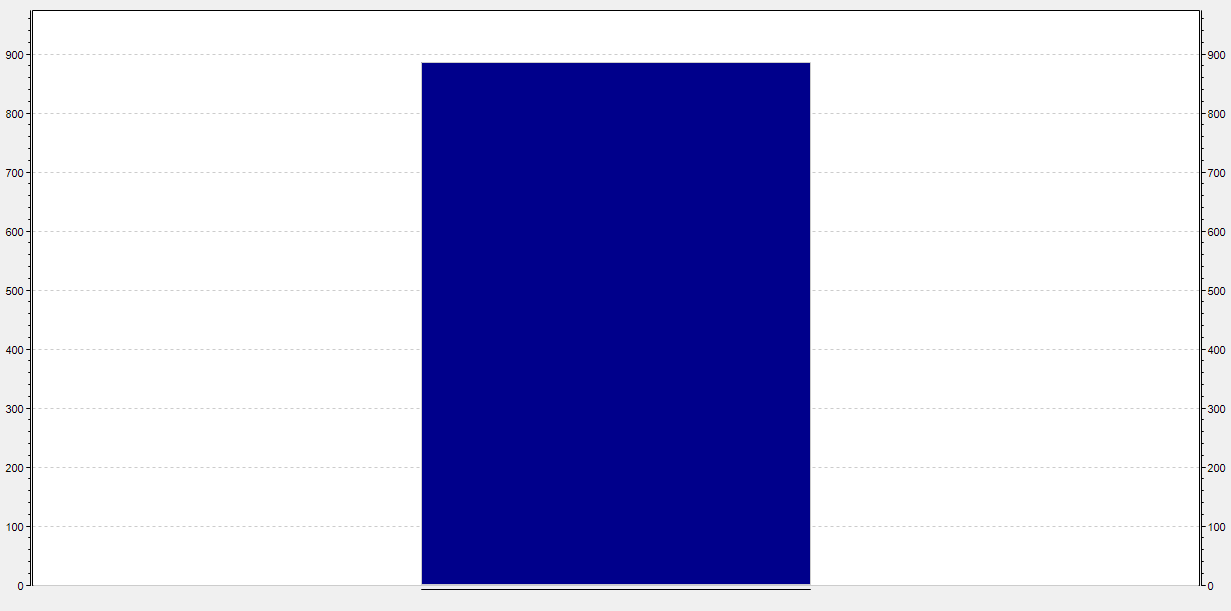
\includegraphics[width=0.30\textwidth]{image/week11/1-2-10.png}
            }\hspace{3mm}
            \caption{Experiment 1-2 Simulation Results Screenshot: 30m, packetReceived}
            \end{figure}
            
    \subsubsection*{1. 2. 3 Discussion}
    \vspace{-3mm}
        결과 분석에 앞서 LTE에서의 modulation coding과 CQI의 관계를 되짚어보자. 아래의 그림은 Release 12 전후의 LTE Modulation and Coding Scheme(MCS)를 나타낸 표이다. LTE에서는 각 단말이 네트워크 상태(SINR)을 측정하고  CQI를 기지국(eNodeB)에 보고한다. CQI가 증가함에 따라 송수신하는 데이터의 Code rate을 계속해서 증가시키고, Modulation 방식을 QPSK, 16QAM, 64QAM, 256QAM 등으로 바꾼다. 그 결과 데이터 전송량, Bits per RE(Resource Element)는 계속해서 증가한다.
        
        시뮬레이션 결과를 다음과 같이 표로 나타냈다.\\
        
        \vspace{-3mm}
        \begin{table}[h!]
        \centering
            \begin{tabular}{|l|l|l|l|l|l|}
            \hline
            \textbf{CQI} & 1 & 3 & 5 & 7 & 9 \\
            \hline
            \multicolumn{1}{|c|}{\textbf{Received Packet(Distance: 25m)}} & \multicolumn{1}{|c|}{283} & 854 & 1507 & 1540 & 1299 \\
            \hline
            \multicolumn{1}{|c|}{\textbf{Received Packet(Distance: 30m)}} & \multicolumn{1}{|c|}{283} & 658 & 1241 & 1353 & 886 \\
            \hline
            \end{tabular}
            \caption{The number of packet received with different CQI}
        \end{table}
        \vspace{-3mm}
        RX가 수신한 packet의 수는 CQI가 1부터 7까지 증가함에 따라 같이 증가하고, CQI가 9에 도달할때 감소한다. CQI가 증가하면서 송수신 하는 데이터(bits per RE)가 증가하고, 수신하는 packet의 수도 역시 증가한다. 하지만 네트워크가 감당할 수 있는 한계를 넘은 CQI로 데이터를 송수신하게 되면, RX에서 데이터 전송 속도를 감당하지 못하고 수신에 실패할 확률이 증가한다. 실험의 TCP D2D(Device-to-Device) 통신은 전송 실패한 packet을 전송 성공할 때까지 재전송하기 때문에 CQI가 한계를 넘어서 증가하면 수신하는 packet의 수가 감소한다. \\
        거리를 25m에서 30m로 증가시키고 실험을 반복했을때, CQI 값이 증가함에 따른 수신한 packet 수의 증감에 대한 경향성은 유사했다. 둘 모두 RX가 수신한 packet의 수가 CQI가 1부터 7까지 증가함에 따라 같이 증가하고, CQI가 9에 도달할때 감소헸다. 하지만 30m의 경우 네트워크 상태가 비교적 나쁘기 때문에 전체적으로 더 적은 packet을 수신했다. 실험 1-1의 결과에서 유추해볼 때, eNodeB와 단말 사이의 거리가 더 증가하면 전체적인 수신한 packet의 수가 감소하고, CQI가 증가함에 따른 수신한 packet의 수가 감소하는 시점은 빨라질 것으로 예상된다.
        \begin{figure}[!h]\centering 
	        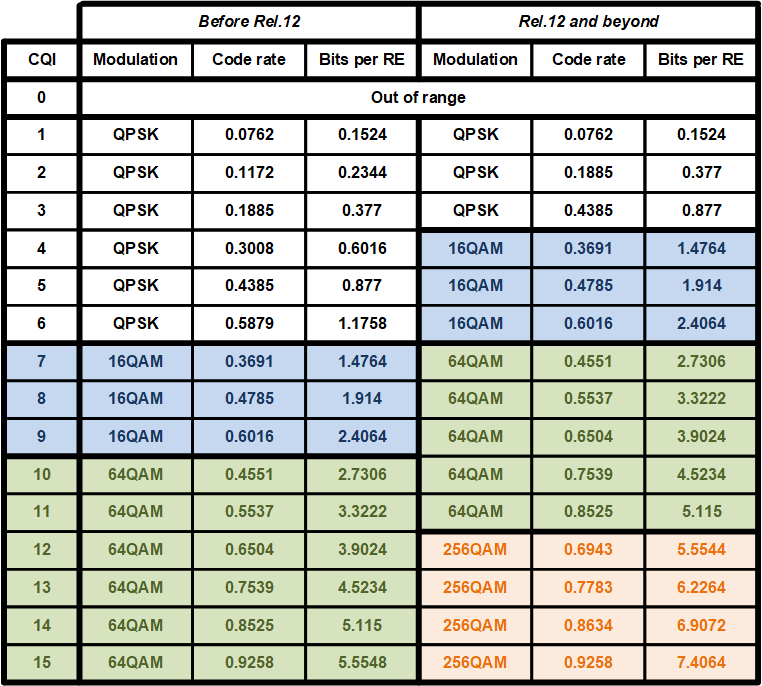
\includegraphics[width=.68\textwidth]{image/week11/1-2-11.png}
	        \caption{\footnotesize
	        Modulation Coding and CQI}
	        \vspace{-10pt}
        \end{figure}